% संपूर्ण मराठी ग्रंथातील प्रकरण 76: संच उपपत्तीचा इतिहास आणि दंतकथा
% हा संपादनयोग्य स्रोतखंड आहे. संकलनासाठी संपूर्ण स्रोतसंग्रहातील
% अक्षररूपे, पूर्वभाग, चिन्हव्याख्या आणि आकृती-स्रोत आवश्यक आहेत.
% मूळ: Open Logic Project; मजकूर आणि रूपांतर CC BY 4.0.
% यंत्रानुवाद, दुरुस्ती आणि तपासणी: OpenAI Codex —
% GPT-5.6 Sol आणि GPT-6 Sol, दोन्ही Ultra effort.
% दुरुस्ती-पुनरावलोकन: GPT-6.1 Sol, Ultra effort.
\chapter{संच उपपत्तीचा इतिहास आणि दंतकथा}\label{his:set:chap}
\begin{editorial}
या प्रकरणात टिम बटन यांच्या Open Set Theory या ग्रंथातील ऐतिहासिक प्रस्तावना
समाविष्ट केली आहे.
\end{editorial}




\section{अतिसूक्ष्म राशी आणि अवकलन}\label{his:set:infinitesimals:sec}

न्यूटन आणि लाइब्निझ यांनी सतराव्या शतकाच्या अखेरीस एकमेकांपासून स्वतंत्रपणे कलनाचा शोध लावला. कलनाचा एक विशेष महत्त्वाचा उपयोग म्हणजे \emph{अवकलन}. ढोबळपणे सांगायचे तर, एखाद्या बिंदूवर फलनाच्या “बदलाचा दर” किंवा उतार निश्चित करणे हा अवकलनाचा उद्देश असतो.

ही कल्पना एका ठळक उदाहरणाने समजते. खाली काळ्या रेषेत दाखवलेले $f(x) = \nicefrac{x^2}{4} + \nicefrac{1}{2}$ हे फलन पाहा:
\begin{center}
	\begin{tikzpicture}[scale=1]
	\draw[->, gray] (-1,0) -- (4.25,0) node[right] {$x$};
	\draw[->, gray] (0,-0.25) -- (0,5.25) node[above] {$f(x)$};

	\foreach \x/\xtext in {1/1, 2/2, 3/3, 4/4}
	\draw[shift={(\x,0)}, gray] (0pt,2pt) -- (0pt,-2pt) node[below] {$\xtext$};

	\foreach \y/\ytext in {1/1, 2/2, 3/3, 4/4, 5/5}
	\draw[shift={(0,\y)}, gray] (2pt,0pt) -- (-2pt,0pt) node[left] {$\ytext$};

	\draw[oldiagcolorC] (0.5, 9/16) -- (3.5, 57/16) -- (3.5, 9/16)--cycle;
	\draw[oldiagcolorD] (.5, 9/16) -- (2.5, 33/16) -- (2.5, 9/16) -- cycle;
	\draw[oldiagcolorE] (.5, 9/16) -- (1.5, 17/16) -- (1.5, 9/16) -- cycle;
	\draw[thick] (-1,.75) parabola bend (0,0.5) (4,4.5);
	\end{tikzpicture}
\end{center}
आपल्याला $c = \nicefrac{1}{2}$ येथे या फलनाचा उतार शोधायचा आहे, असे समजा. प्रथम असा त्रिकोण काढू की त्याचा कर्ण त्या बिंदूवरील उताराचे सन्निकटन देतो; वरील लाल त्रिकोण हे एक उदाहरण आहे. आपल्या त्रिकोणाच्या पायाची लांबी $\beta$ असेल, तर त्याची उंची $f(\nicefrac{1}{2}+\beta) - f(\nicefrac{1}{2})$ असेल. म्हणून कर्णाचा उतार असा मिळतो:
\[
\frac{f(\nicefrac{1}{2}+\beta) - f(\nicefrac{1}{2})}{\beta}.
\]
म्हणून पायाची लांबी~$3$ असलेल्या \textcolor{oldiagcolorC}{लाल} त्रिकोणाचा उतार नेमका~$1$ आहे. त्याहून लहान, पायाची लांबी~$2$ असलेल्या \textcolor{oldiagcolorD}{निळा} त्रिकोणाचा कर्ण अधिक चांगले सन्निकटन देतो; त्याचा उतार $\nicefrac{3}{4}$ आहे. त्याहूनही लहान, पायाची लांबी~$1$ असलेला \textcolor{oldiagcolorE}{हिरवा} त्रिकोण आणखी चांगले सन्निकटन देतो; त्याचा उतार $\nicefrac{1}{2}$ आहे.

त्रिकोण जसजसे लहान होत जातात तसतसे आपल्याला अधिक चांगली सन्निकटने मिळतात. म्हणून आपण असे म्हणू शकू: \emph{अतिसूक्ष्म} पायाची लांबी असलेल्या त्रिकोणाचा कर्ण $c = \nicefrac{1}{2}$ येथील नेमका उतार देतो. अशा रीतीने $c$ या बिंदूवरील $f$ फलनाच्या (पहिल्या) अवकलजाचे सूत्र मिळेल:
\[
{f'}(c) = \frac{f(c+\beta) - f(c)}{\beta} \text{ येथे $\beta$ अतिसूक्ष्म आहे.}
\]
ढोबळपणे पाहता, न्यूटन आणि लाइब्निझ यांचे म्हणणे हेच होते.

मात्र असे म्हटल्यावर आपण त्यांना विचारले पाहिजे: \emph{अतिसूक्ष्म} म्हणजे नेमके काय? येथे एक गंभीर द्विधा निर्माण होते. $\beta = 0$ असेल, तर $f'$ ची व्याख्या नीट होत नाही, कारण त्यात $0$ ने भागाकार करावा लागतो. पण $\beta > 0$ असेल, तर आपल्याला नेमका उतार नव्हे, तर उताराचे \emph{सन्निकटन}च मिळते.

ही नंतरच्या काळातील कल्पना त्या काळावर लादलेली शंका नाही. न्यूटन यांच्या अनुयायांवर टीका करताना बर्कली असे म्हणतात:
\begin{quote}
चिन्हे कोणतीही गोष्ट किंवा काहीच नाही असे दर्शवू शकतात, हे मी मान्य करतो. त्यामुळे मूळ संकेतनातील $c + \beta$ या पदात $\beta$ हे वाढीचे प्रमाण किंवा काहीच नाही, यांपैकी काहीही दर्शवू शकले असते. पण तुम्ही त्याला यांपैकी जो अर्थ द्याल, त्या अर्थाशी सुसंगतपणे युक्तिवाद केला पाहिजे; दुहेरी अर्थाचा आधार घेऊन पुढे जाता कामा नये. तसे करणे म्हणजे उघड कुतर्क होय. (Berkeley 1734, \S{}XIII; आधीच्या मजकुराशी जुळण्यासाठी चल बदलले आहेत.)
\end{quote}
बर्कली यांच्या टीकेपासून अतिसूक्ष्म राशींवरील कलनाचा बचाव करताना, “अतिसूक्ष्म राशी” हा शब्दप्रयोग केवळ रूपकात्मक आहे, असे कोणी म्हणू शकेल. आपण \emph{खरोखर फार लहान} त्रिकोण घेतला, तर स्पर्शरेषेचे \emph{पुरेसे चांगले} सन्निकटन मिळेल, असे त्यांचे म्हणणे असेल. यावरही बर्कली यांचे उत्तर होते: अभियांत्रिकीसाठी ते पुरेसे असेलही, पण त्यामुळे गणिताच्या \emph{स्थानाला} धक्का बसतो; कारण
\begin{quote}
आपल्याला असे सांगितले जाते की \emph{in rebus mathematicis errores qu\`{a}m minimi
non sunt contemnendi}. [गणितात अगदी लहानात लहान चुकाही दुर्लक्षण्याजोग्या नसतात.] (Berkeley 1734, \S{}IX)
\end{quote}
तिरप्या अक्षरांतील हा उतारा न्यूटन यांच्या स्वतःच्या \emph{Quadrature of Curves} (1704) या ग्रंथातील विधानाशी जवळजवळ शब्दशः जुळतो.

बर्कली यांचे तात्त्विक आक्षेप अत्यंत नेमके होते. तरीसुद्धा कलन अत्यंत यशस्वी ठरले आणि गणितज्ञांनी चुका न करता त्याचा वापर चालू ठेवला.












\section{सीमांची काटेकोर व्याख्या}\label{his:set:limits:sec}

आजकाल आधीच्या समस्येवरचे प्रमाणित उत्तर म्हणजे अतिसूक्ष्म राशींचा आधार सोडणे. ते कसे करता येते ते पाहू.

आपण पाहिले की $\beta$ जसजसा लहान होतो तसतशी उताराची अधिक चांगली सन्निकटने मिळतात. खरे तर $\beta$ हा $0$ च्या कितीही जवळ जात असताना, $f'(c)$ या आधीच्या सूत्रातील भागाकाराचा मान आपल्याला हव्या असलेल्या उताराकडे झुकतो. त्यामुळे $\beta = 0$ \emph{असतानाची} स्थिती पाहण्याऐवजी, $\beta$ हा $0$ कडे जात असताना $f'(c)$ च्या त्या सूत्रातील भागाकाराचा \emph{कल} पाहणे पुरेसे आहे.

अशा प्रकारे मांडल्यास, पुढील स्वरूपाच्या विधानांचा अर्थ स्पष्ट करणे हे सर्वसाधारण आव्हान ठरते:
\begin{center}
$x$ हा $c$ कडे जात असताना $g(x)$ चे मूल्य $\ell$ कडे झुकते.
\end{center}
हे अधिक संक्षेपात असे लिहिता येते:
\[
\lim_{x \rightarrow c}g(x) = \ell.
\]
एकोणिसाव्या शतकात कॉशी यांच्या आधीच्या कार्यावर आधार घेत वायेरश्ट्रास यांनी या विधानाची पूर्णपणे काटेकोर व्याख्या दिली. $x$ हा $c$ च्या योग्य इतका जवळ घेतल्यास $g(x)$ हे $\ell$ च्या आपल्याला हवे तितके जवळ नेता येते, हीच त्यामागील कल्पना आहे. अधिक नेमकेपणे, $\lim_{x \rightarrow c} g(x) = \ell$ याचा अर्थ असा ठरवू:
\[
(\forall\epsilon > 0)(\exists \delta > 0)\forall x \left(0 < |x - c| < \delta \lif |g(x) - \ell| < \epsilon \right).
\]

येथील उभ्या रेषा निरपेक्ष मूल्य दर्शवतात. म्हणजे $x \geq 0$ असेल तेव्हा $|x| = x$, आणि $x < 0$ असेल तेव्हा $|x| =-x$; \emph{त्या} फलनाचा आलेख पुढीलप्रमाणे दाखवता येतो:
\begin{center}
	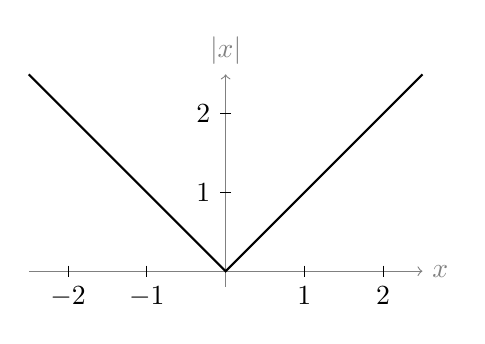
\begin{tikzpicture}[scale=1]
	\draw[->, gray] (-2.5,0) -- (2.5,0) node[right] {$x$};
	\draw[->, gray] (0,-.2) -- (0,2.5) node[above] {$|x|$};

	\foreach \x/\xtext in {-2/-2, -1/-1, 1/1, 2/2}
	\draw[shift={(\x,0)}] (0pt,2pt) -- (0pt,-2pt) node[below] {{$\xtext$}};

	\foreach \y/\ytext in {1/1, 2/2}
	\draw[shift={(0,\y)}] (2pt,0pt) -- (-2pt,0pt) node[left] {{$\ytext$}};

	\draw[thick] (-2.5, 2.5)--(0,0)--(2.5, 2.5);
	\end{tikzpicture}
\end{center}
म्हणून या व्याख्येचा ढोबळ अर्थ असा: $c$ पेक्षा वेगळी पण त्याच्या $\delta$ इतक्या जवळची आदाने निवडून (म्हणजे $0 < |x - c| < \delta$), आपली “त्रुटी” $\epsilon$ पेक्षा लहान करता येते (म्हणजे $|g(x) - \ell| < \epsilon$).

सीमेची संकल्पना व्याख्येने निश्चित केल्यावर आपण अतिसूक्ष्म राशी पूर्णपणे टाळू शकतो. त्यासाठी $c$ येथील $f$ चा उतार असा ठरवू:
\[
	{f}'(c) = \lim_{x \rightarrow 0}\left(\frac{f(c +x) - f(c)}{x}\right) \text{ जेथे सीमा अस्तित्वात आहे}.
\]
मात्र “जेथे सीमा अस्तित्वात आहे” ही अट व्याख्येत का हवी, हे लक्षात घेणे महत्त्वाचे आहे. साधे उदाहरण म्हणून आपण आत्ताच ज्याचा आलेख पाहिला तो $f(x) = |x|$ विचारात घ्या. येथे $f'(0)$ ची व्याख्या होत नाही: $0$ कडे “उजवीकडून” गेल्यास उतार नेहमी $1$ असतो, तर $0$ कडे “डावीकडून” गेल्यास उतार नेहमी $-1$ असतो; म्हणून सीमा अस्तित्वात नाही. त्यामुळे अशी सीमा अस्तित्वात असेल तर आणि तरच फलन~$f$ हे~$x$ येथे \emph{अवकलनीय} आहे, असेही म्हणता येईल.

अवकलनासाठी \emph{सीमेची} संकल्पना कशी वापरायची ते आपण पाहिले. त्याच संकल्पनेने \emph{सतत} फलनाची कल्पनाही व्याख्येने निश्चित करता येते. (१८१७ पर्यंत बोल्झानो यांना हे तत्त्वतः उमगले होते.) कॉशी–वायेरश्ट्रास यांची सातत्याची मांडणी अशी आहे. ढोबळपणे: फलनाच्या निर्गतात ठरावीक अचूकता हवी असेल, तर आदानात पुरेशी अचूकता मागून ती मिळेल, अशा वेळी फलन~$f$ त्या बिंदूवर सतत असते. अधिक नेमकेपणे: $x$ हा शून्याकडे जात असताना $f(c + x)$ आणि $f(c)$ यांतील फरकही $0$ कडे जात असेल, तर $f$ हे $c$ येथे सतत आहे. दुसऱ्या शब्दांत, $f(c) = \lim_{x \rightarrow c} f(x)$ असेल तर आणि तरच $f$ हे $c$ येथे \emph{सतत} आहे.

यापुढे गेलो तर आपला विषय असलेल्या संच उपपत्तीपासून दूर जाऊन आपण वास्तव विश्लेषणात शिरू. म्हणून आता थांबून मुख्य बोध सांगू. एकोणिसाव्या शतकात गणितज्ञांनी काटेकोरपणे व्याख्या केलेल्या \emph{सीमेच्या} संकल्पनेचा वापर करून अतिसूक्ष्म राशींशिवाय काम करायला शिकले.







\section{विलक्षण रचना}\label{his:set:pathology:sec}

मात्र \emph{सीमेच्या} व्याख्येमुळे काही खरोखर “विलक्षण” रचना शक्य असल्याचे दिसून आले.

१८३०च्या सुमारास बोल्झानो यांनी असे एक फलन शोधले जे \emph{सर्वत्र सतत} होते, पण \emph{कोठेही अवकलनीय नव्हते}. (दुर्दैवाने बोल्झानो यांनी हे कधी प्रकाशित केले नाही. वायेरश्ट्रास यांनी स्वतंत्रपणे हीच कल्पना शोधल्यामुळे गणितज्ञांना १८७२ मध्ये तिची प्रथम ओळख झाली.)\footnote{हा इतिहास \href{http://en.wikipedia.org/wiki/Weierstrass_function}{वायेरश्ट्रास फलनावरील विकिपीडिया लेखाच्या} अत्यंत तपशीलवार तळटीपांत नोंदवला आहे.} हे किमान आश्चर्यकारक तरी होतेच. $|x|$ सारखी सर्वत्र सतत, पण एखाद्या विशिष्ट बिंदूवर अवकलनीय नसलेली फलने सहज सापडतात. परंतु सर्वत्र सतत असूनही \emph{कोठेही} अवकलनीय नसलेले फलन अगदी वेगळेच आहे. असे फलन कसे काढाल याचा क्षणभर विचार करा. ते सतत असण्यासाठी कागदावरून लेखणी कधीही न उचलता त्याचा आलेख काढता आला पाहिजे; पण ते कोठेही अवकलनीय नसण्यासाठी लेखणीची दिशा सतत अचानक बदलावी लागेल.

यानंतर आणखी “विलक्षण” रचना समोर आल्या. ५ जानेवारी १८७४ रोजी कँटर यांनी डेडेकिंड यांना पत्र लिहून पुढील प्रश्न विचारला:
\begin{quote}
एखाद्या पृष्ठभागाची (उदाहरणार्थ सीमेसह चौरसाची) एखाद्या रेषेशी (उदाहरणार्थ टोकांसह सरळ रेषेशी) अशी एकास-एक संगती लावता येईल का की पृष्ठभागावरील प्रत्येक बिंदूला रेषेवरील एक बिंदू मिळेल आणि उलट रेषेवरील प्रत्येक बिंदूला पृष्ठभागावरील एक बिंदू मिळेल?

या प्रश्नाचे उत्तर शोधणे अजूनही मला फार कठीण वाटते—तरी येथेही \emph{नाही} असे म्हणण्याची इतकी तीव्र ओढ वाटते की त्यासाठी सिद्धतेची गरज जवळजवळ नसावी असे वाटू लागते.
[Gouv\^{e}a 2011 मधून उद्धृत]
\end{quote}
पण १८७७ मध्ये कँटर यांनी स्वतःचा अंदाज चुकीचा असल्याचे सिद्ध केले. प्रत्यक्षात रेषा आणि चौरस यांवरील बिंदूंची संख्या अगदी सारखी असते. २९ जून १८७७ रोजी त्यांनी डेडेकिंड यांना “\emph{je le vois, mais je ne le crois pas}” असे लिहिले; म्हणजे, “ते मला दिसते, पण त्यावर माझा विश्वास बसत नाही.” गणिताच्या “प्रचलित इतिहासकथनात” याचा अर्थ अनेकदा असा घेतला जातो की त्या काळच्या गणितज्ञांना हे नवे निष्कर्ष \emph{अक्षरशः अविश्वसनीय} वाटत होते. (हा पत्रव्यवहार Gouv\^{e}a (2011) येथे दिला आहे आणि \ref{his:set:mythology:sec} मध्ये आपण त्याकडे पुन्हा वळू. कँटर यांच्या सिद्धतेचा आराखडा \ref{his:set:cantorplane:sec} मध्ये दिला आहे.)

कँटर यांच्या निष्कर्षाने प्रेरित होऊन, एखाद्या रेषेचे \emph{अखंडपणे} प्रतलावर प्रतिचित्रण करून ते प्रतल भरून काढता येईल का, असा विचार पियानो यांनी सुरू केला. असे प्रतिचित्रण म्हणजे \emph{अवकाश भरणारा वक्र} असेल. 1890 मध्ये पियानो यांनी असाच वक्र रचला. हे अंतर्ज्ञानाला खरोखर विरुद्ध वाटते: युक्लिडने रेषेची व्याख्या “रुंदीविरहित लांबी” अशी केली होती (पुस्तक I, व्याख्या २); पण रेषा योग्य प्रकारे वळवली, तर तिची लांबी रुंदी व्यापू शकते, हे पियानो यांनी दाखवले. 1891 मध्ये हिल्बर्ट यांनी याहून किंचित अधिक सहज समजणारा अवकाश भरणारा वक्र आणि त्याची काही चित्रे दिली. हा वक्र टप्प्याटप्प्याने रचला जातो; रचनेचे पहिले सहा टप्पे येथे दिले आहेत:
\begin{center}
\begin{tikzpicture}
\begin{scope}[xshift=20pt, yshift=20pt]
	\draw [oldiagcolorC, l-system={Hilbert curve, step=40pt, angle=90, axiom=L, order=1}] lindenmayer system;
\end{scope}
\begin{scope}[xshift=110pt, yshift=10pt]
	\draw [oldiagcolorC, l-system={Hilbert curve, step=20pt, angle=90, axiom=L, order=2}] lindenmayer system;
\end{scope}
\begin{scope}[xshift=205pt, yshift=5pt]
	\draw [oldiagcolorC, l-system={Hilbert curve, step=10pt, angle=90, axiom=L, order=3}] lindenmayer system;
\end{scope}
\begin{scope}[xshift=2.5pt, yshift=-97.5pt]
	\draw [oldiagcolorC, l-system={Hilbert curve, step=5pt, angle=90, axiom=L, order=4}] lindenmayer system;
\end{scope}
\begin{scope}[xshift=101.25pt, yshift=-98.75pt]
	\draw [oldiagcolorC, l-system={Hilbert curve, step=2.5pt, angle=90, axiom=L, order=5}] lindenmayer system;
\end{scope}
\begin{scope}[xshift=200.625pt, yshift=-99.375pt]
	\draw [oldiagcolorC, l-system={Hilbert curve, step=1.25pt, angle=90, axiom=L, order=6}] lindenmayer system;
\end{scope}
\draw[gray] (0pt,0pt) rectangle (80pt, 80pt);
\draw[gray] (100pt,0pt) rectangle (180pt, 80pt);
\draw[gray] (200pt,0pt) rectangle (280pt, 80pt);
\draw[gray] (0pt,-100pt) rectangle (80pt, -20pt);
\draw[gray] (100pt,-100pt) rectangle (180pt, -20pt);
\draw[gray] (200pt,-100pt) rectangle (280pt, -20pt);
\end{tikzpicture}
\end{center}
सीमेत—जी संकल्पना आता काटेकोरपणे व्याख्यित झाली होती—संपूर्ण चौरस एकसंध \textcolor{oldiagcolorC}{लाल} रंगाने भरतो. तसेच, हिल्बर्ट यांचा वक्र सर्वत्र सतत आहे, पण कोठेही अवकलनीय नाही; अंतर्ज्ञानाने सांगायचे तर, अनंत टप्प्यांच्या सीमेत फलन प्रत्येक क्षणी अचानक दिशा बदलते. (हिल्बर्ट यांच्या रचनेचा अधिक तपशीलवार आराखडा \ref{his:set:hilbertcurve:sec} मध्ये पाहू.)

या “विलक्षण” भूमितीय रचनांना, योग्य की अयोग्य, भूमितीय अंतर्ज्ञानावर विसंबून राहण्याबाबत शंका घेण्याचे कारण मानले गेले. गणित करण्याच्या एका नव्या पद्धतीच्या \emph{प्रचाराचे} त्या जणू साधन बनल्या; या पद्धतीचा विकास पुढे संच उपपत्तीत झाला. या विषयाभोवती नंतर उभ्या राहिलेल्या दंतकथांमध्ये, हे निष्कर्ष पूर्णपणे काटेकोर आणि तितकेच धक्कादायक होते, असे वारंवार सांगितले गेले. त्यामुळे त्यांनी दोन कामे केली: भूमितीय अंतर्ज्ञानावर अवलंबून राहण्याविरुद्ध सावध केले आणि नव्या विचारपद्धतींची फलद्रूपता दाखवली.








\section{इतिहासापेक्षा दंतकथाच अधिक?}\label{his:set:mythology:sec}

या घटनांकडे शतकाहून अधिक काळानंतर मागे वळून पाहताना, त्यांच्याबद्दल प्रचलित झालेले निष्कर्ष विनातपासणी स्वीकारू नयेत. ते गणिती निष्कर्ष नक्कीच नवे, उत्सुकता वाढवणारे आणि आश्चर्यकारक होते. पण ते खरोखर किती धक्कादायक होते? आणि भूमितीय अंतर्ज्ञानावर विसंबू नये, हे त्यांनी खरोखर दाखवले का?

धक्क्याच्या प्रश्नावर Gouv\^{e}a (2011) असे निदर्शनास आणतात की कँटर यांनी डेडेकिंड यांना लिहिलेले प्रसिद्ध “\emph{je le vois, mais je ne le crois
pas}” हे वाक्य त्याच्या संदर्भातून बरेचसे वेगळे केले जाते. तो संदर्भ पुढे दिला आहे (Gouv\^{e}a यांच्याकडून उद्धृत):
\begin{quote}
या विषयाबद्दलच्या माझ्या उत्साहापोटी मी तुमच्या दयाळूपणाची आणि संयमाची इतकी मागणी करत असेन, तर मला क्षमा करा. मी तुम्हाला अलीकडे पाठवलेले विचार मलाही इतके अनपेक्षित, इतके नवे वाटतात की, आदरणीय मित्रा, त्यांची अचूकता तुम्ही निश्चित करेपर्यंत मला मनःशांती मिळू शकत नाही. तुम्ही माझ्याशी सहमत होत नाही तोपर्यंत मी एवढेच म्हणू शकतो:
\emph{je le vois, mais je ne le crois pas.}
\end{quote}
आपला निष्कर्ष “इतका अनपेक्षित, इतका नवा” आहे हे कँटर यांना माहीत होते. पण तो निष्कर्ष त्यांना खरोखर \emph{अविश्वसनीय} वाटत होता का, याबद्दल शंका आहे. Gouv\^{e}a यांनी दाखवल्याप्रमाणे, त्यांनी डेडेकिंड यांना केवळ स्वतः दिलेल्या सिद्धतेची तपासणी करायला सांगितले होते.

भूमितीय अंतर्ज्ञानाच्या प्रश्नावर पाहिले तर, पियानो यांनी अवकाश भरणारा वक्र प्रकाशित करताना कोणतीही चित्रे दिली नव्हती. पण हिल्बर्ट यांनी स्वतःचा वक्र प्रकाशित केला तेव्हा आपला हेतू त्यांनी स्पष्ट केला: वाचकांनी “पुढील भूमितीय अंतर्ज्ञानाचा आधार घेतल्यास” पियानो यांचा निष्कर्ष त्यांना नीट समजावा, म्हणून त्यांनी \ref{his:set:pathology:sec} मध्ये दिलेल्यांसारखी \emph{चित्रे} त्यात जोडली.

अधिक सर्वसाधारणपणे सांगायचे तर, प्रकाशित सिद्धतांमध्ये चित्रे वापरण्याची पद्धत काहीशी कमी झाली असली तरी गणितज्ञ सिद्धता करताना \emph{वारंवार} चित्रे वापरतात, ही गोष्ट नाकारता येत नाही. (ढोबळपणे सांगायचे तर, भूमितीय अंतर्ज्ञानावर कधी विसंबता येते हे चांगल्या गणितज्ञांना माहीत असते.)

थोडक्यात, अतिरंजित प्रचारावर विश्वास ठेवू नका; निदान तो विनातपासणी स्वीकारू नका. याबद्दल अधिक माहितीसाठी Giaquinto (2007) वाचता येईल.








\section{रेषा आणि प्रतल: कँटर यांचा निष्कर्ष}\label{his:set:cantorplane:sec}

श्रेडर--बर्नस्टाइन प्रमेयाच्या सिद्धतेशी संबंधित काही परिस्थितींचा संबंध \ref{his:set:pathology:sec} मध्ये चर्चिलेल्या इतिहासाशी आहे. आठवा: १८७७ मध्ये कँटर यांनी चौरसावर जितके बिंदू आहेत तितकेच त्याच्या एका बाजूवरही आहेत, हे सिद्ध केले. त्यांच्या सुरुवातीच्या प्रयत्नातील अंक एकाआड एक लिहिण्याची कल्पना येथे द्विमान रूपात मांडू. मूळ ऐतिहासिक प्रयत्न दशमान विस्तारांवर आधारलेला होता; खालील द्विमान मांडणी ही त्याचे आधुनिक रूपांतर आहे ((Gouv\^{e}a 2011, पृ.~201--202)).

$\unitline$ ही एकक रेषा, म्हणजे $[0,1]$ या बिंदूंचा संच, असू द्या. $\unitsquare$ हा एकक चौरस, म्हणजे $\unitline \times \unitline$ या बिंदूंचा संच, असू द्या. या संज्ञांत कँटर यांनी $\cardeq{\unitline}{\unitsquare}$ सिद्ध केले. त्यांनी डेडेकिंड यांना पत्रातून कळवलेल्या कल्पनेचे द्विमान रूपांतर पुढे दिले आहे.

\begin{thm}\label{his:set:cantorplane:thm:cantorplane}
$\cardeq{\unitline}{\unitsquare}$
\end{thm}

\begin{proof}[सिद्धता: पहिला भाग.]
$a,b\in\unitline$ निश्चित करा. द्विमान विस्तारासाठी पुढील
एकच पद्धत ठरवू: $0=0.000\ldots$; दोन निरूपणे असलेल्या
धन संख्येसाठी शेवटी अनंत $1$ असलेले निरूपण वापरू.
विशेषतः $\nicefrac12=0.0111\ldots$ आणि $1=0.111\ldots$.
इतर संख्येचे द्विमान निरूपण एकमेव असते. या निवडीने
प्रत्येक धन संख्येच्या विस्तारात अनंत $1$ येतात. असे लिहा:
\begin{align*}
a &= 0.a_1a_2a_3a_4\dots\\
b &= 0.b_1b_2b_3b_4\dots
\intertext{आता पुढीलप्रमाणे दिलेले $f\colon\unitsquare\to\unitline$ हे फलन विचारात घ्या:}
f(a,b)&=0.a_1b_1a_2b_2a_3b_3a_4b_4\dots
\end{align*}
परिणामी विस्तारात अनंत $1$ असतात, जोपर्यंत $a=b=0$
नाहीत; त्या प्रकरणात तो पूर्णपणे शून्यांचा असतो.
म्हणून परिणामी विस्तारही वर ठरवलेल्या पद्धतीतीलच आहे.
त्याच्या अंकांचे एकमेवपण वापरल्यास, $f(a,b)=f(c,d)$
असताना प्रत्येक $n\in\Nat$ साठी $a_n=c_n$ आणि
$b_n=d_n$ मिळते. म्हणून $a=c$ आणि $b=d$;
म्हणजे $f$ हे एकास-एक फलन आहे.
\end{proof}

मात्र हे फलन आच्छादक फलन नाही. उदाहरणार्थ,
द्विमान संख्या $z=0.1101010101\ldots=\nicefrac56$ घ्या.
तिचा द्विमान विस्तार सांत नाही, म्हणून त्या विस्ताराची दुसरी
निवड उपलब्ध नाही. $f(a,b)=z$ असते, तर तिचे विषम आणि
सम स्थानांवरील अंक वेगळे केल्याने अनुक्रमे
\begin{align*}
a&=0.100000\ldots=\nicefrac12,\\
b&=0.111111\ldots=1
\end{align*}
असे विस्तार मिळाले असते. पण $a$ चा हा विस्तार आपण
ठरवलेल्या पद्धतीला मान्य नाही: $\nicefrac12$ साठी
$0.011111\ldots$ वापरायचा आहे. त्यामुळे $z$ साठी
कोणतीही जोडी $\tuple{a,b}$ मिळत नाही.
उदाहरणार्थ, $0.101010\ldots$ हा मात्र
या पद्धतीत $f(1,0)$ आहे; म्हणून तो येथे प्रतिउदाहरण नाही.

अंक एकाआड एक लिहिण्याच्या ऐतिहासिक प्रयत्नात
निरूपणांची निवड महत्त्वाची आहे, हे डेडेकिंड यांनी
निदर्शनास आणले. वरच्या निश्चित द्विमान पद्धतीत $f$
हे एकास-एक फलन आहे, पण आच्छादक फलन नाही.
म्हणून या पहिल्या भागाने फक्त
$\cardle{\unitsquare}{\unitline}$ दाखवले आहे;
$\cardeq{\unitsquare}{\unitline}$ अजून सिद्ध झालेले नाही.

कँटर यांनी डेडेकिंड यांना जवळजवळ लगेच उत्तर लिहून सिद्धता साधारणपणे पुढीलप्रमाणे पूर्ण करता येईल असे सुचवले:

\begin{proof}[सिद्धता: पूर्ण रूप.]
आपण $\cardle{\unitsquare}{\unitline}$ दाखवले आहे. पण $\unitline$ वरून $\unitsquare$ मध्ये जाणारे एकास-एक फलन उघडच आहे: रेषा चौरसाच्या एका बाजूवर सरळ ठेवा. म्हणून $\cardle{\unitline}{\unitsquare}$ आणि $\cardle{\unitsquare}{\unitline}$. श्रेडर--बर्नस्टाइन प्रमेयानुसार (\ref{sfr:siz:sb:thm:schroder-bernstein}) $\cardeq{\unitline}{\unitsquare}$.
\end{proof}

मात्र कँटर यांना अर्थातच शेवटची ओळ या रूपात पूर्ण करता आली नसती, कारण श्रेडर--बर्नस्टाइन प्रमेय तेव्हा अजून सिद्ध झाले नव्हते. पुढे कँटर यांनी हा सर्वसाधारण अंदाज मांडला, तरी त्याची समाधानकारक सिद्धता १८९७ पर्यंत मिळाली नव्हती. (म्हणूनच १८७७ मध्ये पुढे कँटर यांनी \ref{his:set:cantorplane:thm:cantorplane} ची श्रेडर--बर्नस्टाइन प्रमेयाचा आधार न घेणारी वेगळी सिद्धता दिली.)









\section{परिशिष्ट: हिल्बर्ट यांचे अवकाश भरणारे वक्र}\label{his:set:hilbertcurve:sec}

रेषा आणि चौरस यांवर नेमके सारखेच बिंदू असतात, या कँटर यांच्या सिद्धतेमुळे (\ref{his:set:cantorplane:thm:cantorplane}) अवकाश भरणारा \emph{वक्र} असू शकेल का, हा प्रश्न पियानो यांना कसा पडला, याचा उल्लेख आपण \ref{his:set:pathology:sec} मध्ये केला होता. १८९० मध्ये पियानो यांना त्याचे होकारार्थी उत्तर मिळाले. या विभागात हिल्बर्ट यांचा अवकाश भरणारा वक्र (एका लहानशा बदलासह) कसा रचता येतो, हे अनौपचारिक रीतीने स्पष्ट करू.\footnote{अधिक काटेकोर स्पष्टीकरणासाठी (Rose 2010) पाहा. या बदलात खालील वक्रांचे लाल भाग समाविष्ट केले आहेत. त्यामुळे वक्र सतत आहे हे तपासणे थोडे सोपे होते.}

$h$ हे फलन $h_1$, $h_2$, $h_3$, \dots\@ या फलन-अनुक्रमाची सीमा म्हणून व्याख्यित करायचे आहे. प्रथम रचनेचे वर्णन करू. मग ती रचना अवकाश भरते हे दाखवू. त्यानंतर ती खरोखर वक्र आहे हे दाखवू.

$h$ चा लक्ष्यसंच एकक चौरस $\unitsquare$ घेऊ. $h$ चे पहिले सन्निकटन, म्हणजे $h_1$, असे दिसते:
\begin{center}
	\begin{tikzpicture}
	\draw[gray] (0pt, 0pt) rectangle (80pt, 80pt);
	\draw[step = 40pt, gray, very thin] (0pt, 0pt) grid (80pt, 80pt);
	\draw[oldiagcolorC, thick] (20pt, 0)--(20pt, 20pt);
	\draw[oldiagcolorC, thick] (60pt, 0)--(60pt, 20pt);
	\begin{scope}[xshift=20pt, yshift=20pt]
	\draw [black, thick, l-system={Hilbert curve, step=40pt, angle=90, axiom=L, order=1}]  lindenmayer system;
	\end{scope}
	\end{tikzpicture}
\end{center}
रचनेचा मागोवा घेण्यासाठी चौरसावर $2 \times 2$ जाळी आखली आहे. वक्राची सुरुवात खालच्या डाव्या चतुर्थांशात होते, तो वरच्या डाव्या, मग वरच्या उजव्या आणि शेवटी खालच्या उजव्या चतुर्थांशात जातो, असे मानता येते. रचनेचा दुसरा टप्पा, म्हणजे $h_2$, असा आहे:
\begin{center}
	\begin{tikzpicture}
	\draw[gray] (0pt, 0pt) rectangle (80pt, 80pt);
	\draw[step = 20pt, gray, very thin] (0pt, 0pt) grid (80pt, 80pt);
	\draw[oldiagcolorC, thick] (0pt, 10pt)--(10pt, 10pt);
	\draw[oldiagcolorC, thick] (70pt, 10pt)--(80pt, 10pt);
	\draw[thick, oldiagcolorE] (10pt, 30pt)--(10pt, 50pt);
	\draw[thick, oldiagcolorE] (30pt, 50pt)--(50pt, 50pt);
	\draw[thick, oldiagcolorE] (70pt, 50pt)--(70pt, 30pt); \begin{scope}[xshift=10pt, yshift=30pt]
	\draw [thick, rotate=270,black, l-system={Hilbert curve, step=20pt, angle=90, axiom=L, order=1}]  lindenmayer system;
	\end{scope}
	\begin{scope}[xshift=10pt, yshift=50pt]
	\draw [thick, black, l-system={Hilbert curve, step=20pt, angle=90, axiom=L, order=1}]  lindenmayer system;
	\end{scope}
	\begin{scope}[xshift=50pt, yshift=50pt]
	\draw [thick, black, l-system={Hilbert curve, step=20pt, angle=90, axiom=L, order=1}]  lindenmayer system;
	\end{scope}
	\begin{scope}[xshift=70pt, yshift=10pt]
	\draw [thick, rotate=90,black, l-system={Hilbert curve, step=20pt, angle=90, axiom=L, order=1}]  lindenmayer system;
	\end{scope}
	\end{tikzpicture}
\end{center}
$h_2$ कसा रचला ते वेगवेगळ्या रंगांमुळे स्पष्ट होते. प्रथम $h_1$ च्या \textcolor{oldiagcolorC}{लाल} नसलेल्या भागाच्या लहान प्रमाणातील प्रती चौरसाच्या खालच्या डाव्या, वरच्या डाव्या, वरच्या उजव्या आणि खालच्या उजव्या भागांत ठेवतो (त्या काळ्या रंगात दाखवल्या आहेत). मग या चार आकृत्या एकमेकांना (\textcolor{oldiagcolorE}{हिरवा} रेषांनी) जोडतो. शेवटी संपूर्ण आकृती चौरसाच्या सीमेला (\textcolor{oldiagcolorC}{लाल} रेषांनी) जोडतो.

आता $h_3$ पाहू. $h_1$ च्या लाल नसलेल्या भागाच्या एकमेकांना जोडलेल्या चार लहान प्रती वापरून $h_2$ जसा तयार केला, तसाच $h_2$ च्या लाल नसलेल्या भागाच्या चार लहान प्रतींमधून $h_3$ तयार होतो (प्रती काळ्या रंगात दाखवल्या आहेत). नंतर त्या (\textcolor{oldiagcolorE}{हिरवा} रेषांनी) जोडल्या जातात आणि शेवटी चौरसाच्या सीमेला (\textcolor{oldiagcolorC}{लाल} रेषांनी) जोडल्या जातात.
\begin{center}
	\begin{tikzpicture}
	\draw[gray] (0pt, 0pt) rectangle (80pt, 80pt);
	\draw[step = 10pt, gray, very thin] (0pt, 0pt) grid (80pt, 80pt);
	\draw[thick, oldiagcolorC](5pt, 0pt)--(5pt, 5pt);
	\draw[thick, oldiagcolorC] (75pt, 0pt)--(75pt, 5pt);
	\draw[thick, oldiagcolorE] (75pt, 45pt)--(75pt, 35pt);
	\draw[thick, oldiagcolorE] (5pt, 35pt)--(5pt, 45pt);
	\draw[thick, oldiagcolorE] (35pt, 45pt)--(45pt, 45pt);
	\draw[thick, oldiagcolorE] (75pt, 45pt)--(75pt, 35pt); \begin{scope}[xshift=5pt, yshift=35pt]
	\draw [rotate=270, thick, black, l-system={Hilbert curve, step=10pt, angle=90, axiom=L, order=2}]  lindenmayer system;
	\end{scope}
	\begin{scope}[xshift=5pt, yshift=45pt]
	\draw [thick, black, l-system={Hilbert curve, step=10pt, angle=90, axiom=L, order=2}]  lindenmayer system;
	\end{scope}
	\begin{scope}[xshift=45pt, yshift=45pt]
	\draw [thick, black, l-system={Hilbert curve, step=10pt, angle=90, axiom=L, order=2}]  lindenmayer system;
	\end{scope}
	\begin{scope}[xshift=75pt, yshift=5pt]
	\draw [thick, rotate=90,black, l-system={Hilbert curve, step=10pt, angle=90, axiom=L, order=2}]  lindenmayer system;
	\end{scope}
	\end{tikzpicture}
\end{center}
आता सर्व टप्प्यांतील प्राचल सुसंगतपणे ठरवू.
$h_n$ भेट देतो त्या क्रमाने बंद जाळी-घरे
$Q_{n,0},\ldots,Q_{n,4^n-1}$ म्हणा. प्रत्येक घरासाठी
एकक अंतरालाचा समान लांबीचा भाग
\[
I_{n,k}=\left[\frac{k}{4^n},\frac{k+1}{4^n}\right]
\qquad(0\leq k<4^n)
\]
वापरू. या भागाच्या पहिल्या अर्ध्यावर घराच्या प्रवेशबिंदूपासून
मध्यबिंदूपर्यंत आणि दुसऱ्या अर्ध्यावर मध्यबिंदूपासून
निर्गमबिंदूपर्यंत रेषीय रीतीने जाऊ. लागोपाठच्या घरांचा
निर्गम आणि प्रवेश त्यांच्या सामायिक बाजूचा मध्यबिंदू
असतो; संपूर्ण मार्गाचे पहिले आणि शेवटचे बिंदू आकृत्यांतील
लाल भागांच्या बाह्य टोकांवर असतात. त्यामुळे हेच रेखाखंड
मिळतात आणि प्रत्येक $h_n\colon\unitline\to\unitsquare$
सतत असतो.
आकृत्यांतील फिरवलेल्या लहान प्रतींचा क्रम पुनरावृत्तीने
वापरतो: $I_{n,k}$ चे चार समान उपभाग पुढील टप्प्यात
$Q_{n,k}$ च्या चार उपघरांना त्याच भेटीच्या क्रमाने
जोडले जातात. म्हणून प्रत्येक $m\geq n$ साठी
\[
h_m(I_{n,k})\subseteq Q_{n,k}.
\]
येथे बंद घरे वापरली आहेत; अंतरालांचे सामायिक टोक दोन्ही
संबंधित घरांच्या सामायिक सीमेतच जाते.
प्रत्येक $Q_{n,k}$ च्या कर्णाची लांबी
\[
D_n=\sqrt{\left(\nicefrac{1}{2^{n}}\right)^2+
\left(\nicefrac{1}{2^{n}}\right)^2}
=2^{(\frac{1}{2}-n)}
\]
असते. $x\in I_{n,k}$ घेतल्यास $h_m(x)$ आणि $h_n(x)$
हे दोन्ही $Q_{n,k}$ मध्ये आहेत. त्यामुळे
\[
\sup_{x\in\unitline}\|h_m(x)-h_n(x)\|\leq D_n
\qquad(m\geq n).
\]
$D_n\to0$ आणि $\Real^2$ पूर्ण असल्याने प्रत्येक
$x\in\unitline$ साठी $h_n(x)$ ची सीमा अस्तित्वात आहे.
म्हणून
\[
h(x)=\lim_{n\to\infty}h_n(x)
\]
असे व्याख्यित करू शकतो. शिवाय
$\|h(x)-h_n(x)\|\leq D_n$ सर्व $x$ साठी असल्याने
हे अभिसरण समसमान आहे; बंद घरात सीमा घेतल्याने
$h(I_{n,k})\subseteq Q_{n,k}$ सुद्धा मिळते.

आता $h$ अवकाश भरतो हे दाखवू. $p\in\unitsquare$ घ्या.
$p$ धारण करणारे पहिले जाळी-घर निवडा, मग प्रत्येक
टप्प्यात त्याचे $p$ धारण करणारे उपघर निवडा. या
घरांना जोडलेले $I_{n,k_n}$ हे एकमेकांत अंतर्भूत,
रिकामे नसलेले बंद अंतराल आहेत आणि त्यांच्या लांबी
$4^{-n}\to0$ होतात. त्यांच्या छेदात एक बिंदू $x$
असतो. प्रत्येक $n$ साठी $h(x)$ आणि $p$ हे दोन्ही
$Q_{n,k_n}$ मध्ये असल्याने $\|h(x)-p\|\leq D_n$.
$D_n\to0$ म्हणून $h(x)=p$. अशा प्रकारे
$h(\unitline)=\unitsquare$.


आता $h$ हा खरोखर \emph{वक्र} आहे हे दाखवायचे आहे. त्यासाठी वक्राची संकल्पना व्याख्यित करावी लागेल. आधुनिक व्याख्या १८८७ मध्ये जॉर्डन यांनी दिलेल्या व्याख्येवर आधारलेली आहे (म्हणजे पहिला अवकाश भरणारा वक्र येण्याच्या अवघ्या काही वर्षांपूर्वीची).

\begin{defn}
वक्र म्हणजे $\unitline$ वरून $\Real^2$ मध्ये जाणारे सतत फलन.
\end{defn}

ही कल्पना बरीच सहज समजते: वक्र एकक रेषेचे बिंदू
प्रतलातील बिंदूंमध्ये सतत रीतीने पाठवतो. आपले $h$ हे
$\unitline$ वरून $\Real^2$ मध्ये जाणारे फलन आहे.
म्हणून $h$ सतत आहे हेच दाखवायचे उरते.
\ref{his:set:limits:sec} मधील $\epsilon$/$\delta$ व्याख्येनुसार,
प्रत्येक $x_0\in\unitline$ आणि $\epsilon>0$ साठी
असा $\delta>0$ मिळायला हवा की
$x\in\unitline$ आणि $|x-x_0|<\delta$ असल्यास
$\|h(x)-h(x_0)\|<\epsilon$.
अंतरालाच्या टोकांवरही शेजार $\unitline$ च्या सापेक्ष
घ्यायचा आहे.

$x_0$ आणि $\epsilon>0$ निश्चित करा.
$D_n<\epsilon/3$ होईल असा $n$ घ्या.
$h_n$ हा सतत बहुभुजी मार्ग असल्याने असा $\delta>0$
मिळतो की $x\in\unitline$ आणि $|x-x_0|<\delta$
असताना $\|h_n(x)-h_n(x_0)\|<\epsilon/3$.

त्या $x$ साठी त्रिकोण-असमानतेने
\begin{align*}
\|h(x)-h(x_0)\|
&\leq\|h(x)-h_n(x)\|+\|h_n(x)-h_n(x_0)\|
+\|h_n(x_0)-h(x_0)\|\\
&\leq D_n+\|h_n(x)-h_n(x_0)\|+D_n
<\epsilon.
\end{align*}
म्हणून $h$ प्रत्येक $x_0$ येथे सतत आहे आणि व्याख्येनुसार
एक वक्र आहे. आधी सिद्ध केलेल्या
$h(\unitline)=\unitsquare$ मुळे तो अवकाश भरणारा वक्र आहे.





\part{संदर्भसामग्री}\label{ref:part}
\begin{editorial}
  या भागात पाठ्यपुस्तकाच्या परिशिष्टांत समाविष्ट करण्यासाठी वर्णमाला,
  संकेतपद्धती, व्याख्या, नियम इत्यादींच्या विविध याद्या एकत्र केल्या आहेत.
\end{editorial}
